% results.tex
\documentclass[main.tex]{subfiles}
\begin{document}
\chapter{Results} \label{ch:res}

This chapter presents all the experimental results from the procedures described in Chapter \ref{ch:exp}, as well as describing in detail the proper data processing that leads to development of the desired failure surface.

\section{Tensile Tests} \label{sec:tensr}
Performing tensile tests showed that the values of $X_t$ and $Y_t$ were significantly different, in accordance to the literature review presented in Section \ref{ssec:mechPropFFF}. An initial number of 20 samples per orientation was produced, however, multiple specimens failed outside the gage section of the coupon and thus, data that stemmed from these samples was considered invalid and promptly discarded. The valid results are summarized in Table \ref{tab:tensrtab}. Note that $X_t$ was on average 9.16 MPa higher than $Y_t$, a difference of 22.7\%.
\begin{table} [h]
	\centering
	\caption{Summary of Tensile tests}
\begin{tabular}{ c| c c } 
	\toprule
	\textbf{Information} & $X_t$ & $Y_t$\\
	\midrule
	Average [MPa] & 40.29 & 31.13\\
	Standard Deviation & 0.75 & 0.58\\
	Number of samples & 19 & 12\\
	\bottomrule
\end{tabular}
\label{tab:tensrtab}
\end{table}

The behavior of both sets of samples was completely different. Coupons used to measure $X_t$ generally clearly showed whitening of the gage section, indicating plastic deformation. Specimens used for $Y_t$ on the other hand generally failed between beads and rarely showed any change of color. Figure~\ref{fig:tensComp} clearly shows the difference in mechanical behavior. Note how specimens printed with 0$^\circ$ show a clearly ductile failure, as opposed to brittle failure for samples 90$^\circ$ orientation.

\begin{figure}[h]
	\center
	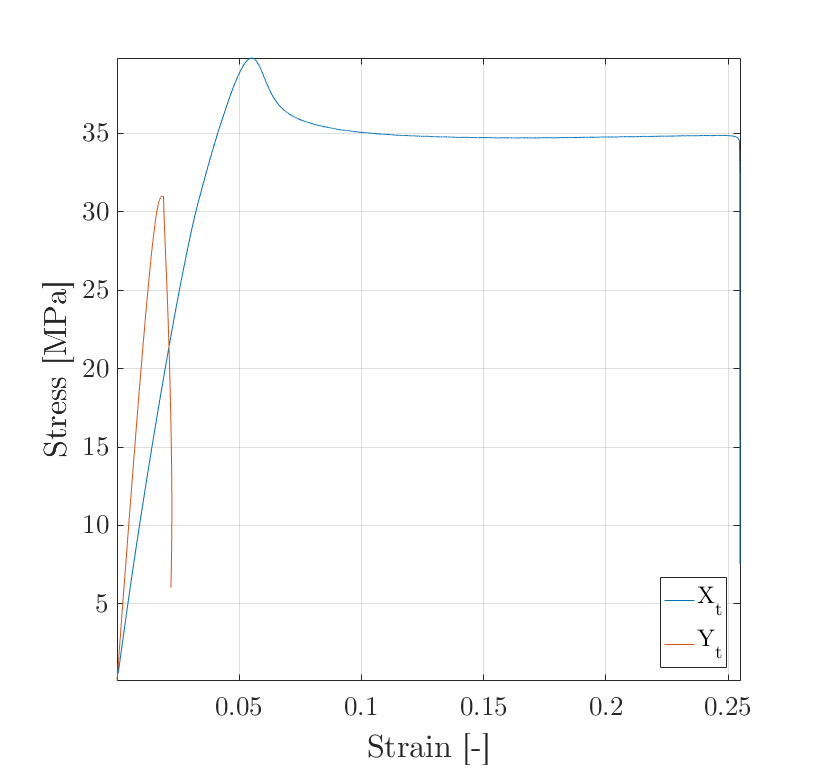
\includegraphics[height=9cm, keepaspectratio]{tenscomp}
	\caption{Comparison of tensile results} \label{fig:tensComp}
\end{figure}

\section{Compression Tests} \label{sec:compr}
\begin{table} [h]
	\centering
	\caption{Summary of Compression tests}
	\begin{tabular}{ c| c c } 
		\toprule
		\textbf{Information} & $X_c$ & $Y_c$\\
		\midrule
		Average [MPa] &  & 58.8\\
		Standard Deviation &  & 1.90\\
		Number of samples &  & 15\\
		\bottomrule
	\end{tabular}
\label{tab:comprtab}
\end{table}

\section{Torsion Tests} \label{sec:torsr}
\subsection{45$^\circ$ orientation} \label{ssec:45r}
\subsection{0$^\circ$ orientation} \label{ssec:0r}
\subsection{90$^\circ$ orientation} \label{ssec:90r}
\section{Combined Loading Tests} \label{sec:clr}
\section{Development of the Failure Surface} \label{sec:fsc}
% Nomenclature introduced in this chapter:
%\nomenclature[A]{ABS}{Acrylonitrile Butadiene Styrene}% 

% Symbols introduced in this chapter:
%\nomenclature[S]{$\epsilon$}{Engineering Strain \nomunit{$-$}}%
\end{document}